\subsection{Interpreter}
\label{interpreter}

\textbf{Scopo}: Comportamentale \\
\textbf{Raggio d'azione}: Oggetti

\paragraph{Definizione} Il pattern Interpreter è un modello di progettazione che fornisce un modo per interpretare e valutare espressioni di un linguaggio, rappresentando la grammatica tramite una gerarchia di classi. Ogni classe corrisponde a una regola della grammatica e consente di comporre espressioni complesse in modo gerarchico.

Si definiscono classi di espressioni terminali (elementi di base) e non terminali (combinazioni di elementi), organizzate in una struttura ad albero simile al pattern Composite.

\begin{figure}[H]
    \centering
    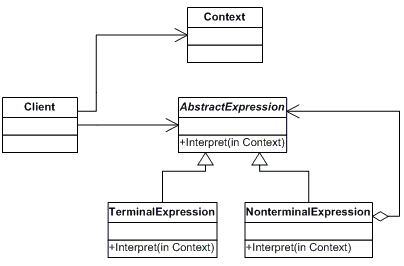
\includegraphics[width=1\linewidth]{assets/pattern/interpreter/interpreter-struttura.png}
    \caption{Class Diagram del pattern Interpreter}
\end{figure}

\paragraph{Struttura e Conseguenze} Il pattern comprende:
\begin{itemize}
    \item \textbf{AbstractExpression}: Interfaccia o classe astratta che dichiara il metodo \texttt{interpreta}, comune a tutte le espressioni.
    \item \textbf{TerminalExpression}: Classi concrete che rappresentano i simboli di base della grammatica (foglie dell'albero), come numeri o variabili.
    \item \textbf{NonterminalExpression}: Classi concrete che rappresentano combinazioni di espressioni e gestiscono la logica di interpretazione delle sottoespressioni.
\end{itemize}

Le espressioni non terminali coordinano l'interpretazione delle sottoespressioni, aggregando i risultati per ottenere il valore finale dell'espressione.

\textbf{Vantaggi}:
\begin{itemize}
    \item Semplicità di implementazione: facilita la definizione e interpretazione di linguaggi semplici, rendendo il codice leggibile e manutenibile.
    \item Estensibilità: aggiungere nuove regole grammaticali è semplice, basta creare nuove classi.
\end{itemize}

\textbf{Svantaggi}:
\begin{itemize}
    \item Complessità: per linguaggi complessi, l'albero sintattico può diventare grande e difficile da gestire.
    \item Performance: la creazione e interpretazione degli alberi può essere inefficiente per linguaggi articolati.
\end{itemize}

\newpage
